\documentclass[11pt]{article}
\usepackage[hmargin=1in,vmargin=1in]{geometry}
\usepackage{xcolor}
\usepackage{amsmath,amssymb,amsfonts,url,sectsty,framed,tcolorbox,framed}
\newcommand{\pf}{{\bf Proof: }}
\newtheorem{theorem}{Theorem}
\newtheorem{lemma}{Lemma}
\newtheorem{proposition}{Proposition}
\newtheorem{definition}{Definition}
\newtheorem{remark}{Remark}
\newcommand{\qed}{\hfill \rule{2mm}{2mm}}
\newtheorem{example}{Example}
\usepackage{tikz}
\usepackage{bm}

\begin{document}
%%%%%%%%%%%%%%%%%%%%%%%%%%%%%%%%%%%%%%%%%%%%%%%%%%%%%%%%%%%%%%%%%%%%%
\noindent
\rule{\textwidth}{1pt}
\begin{center}
{\bf [CS304] Introduction to Cryptography and Network Security}
\end{center}
Course Instructor: Dr. Dibyendu Roy \hfill Winter 2023-2024\\
Scribed by: Raghav Agiwal (202151124) \hfill Lecture (Week 9)
\\
\rule{\textwidth}{1pt}
%%%%%%%%%%%%%%%%%%%%%%%%%%%%%%%%%%%%%%%%%%%%%%%s%%%%%%%%%%%%
%write here


\section{Public Key Cryptography}

Public-key cryptography, also known as asymmetric cryptography, involves using pairs of related keys to encrypt and decrypt data. Each key pair comprises a public key and a corresponding private key.

\subsection*{How It Works}

\begin{enumerate}
    \item \textbf{Key Generation}: A user generates a key pair using cryptographic algorithms. This process involves creating a public key $K_{\text{public}}$ and a private key $K_{\text{private}}$. These keys are mathematically related but computationally infeasible to derive one from the other.
    
    \item \textbf{Public Key Distribution}: The public key is made freely available to anyone who wants to send encrypted messages or verify the sender's identity. It can be shared openly without compromising security.
    
    \item \textbf{Private Key Security}: The private key, on the other hand, is kept secret and known only to the owner. It is used for decrypting messages encrypted with the corresponding public key and for digitally signing messages.
    
    \item \textbf{Encryption}: If someone wants to send an encrypted message to the owner of a public key, they use that public key to encrypt the message. Once encrypted, only the corresponding private key can decrypt it.
    
    \item \textbf{Digital Signatures}: Public key cryptography is also used for creating digital signatures. A digital signature is created by encrypting a message or its hash value with the sender's private key. The recipient can then verify the signature using the sender's public key, ensuring the message hasn't been altered and originated from the claimed sender.
    
    \item \textbf{Security Strength}: Public key cryptography relies on mathematical problems, such as factoring large numbers or calculating discrete logarithms, which are computationally difficult to solve. The security of the system depends on the complexity of these mathematical problems.
\end{enumerate}

\subsection{Diffie-Hellman Key Exchange Algorithm}

The Diffie-Hellman key exchange algorithm is a method used to securely establish a shared secret key between two parties over an insecure communication channel. It was developed independently by Whitfield Diffie and Martin Hellman in 1976 and is one of the earliest practical examples of public-key cryptography.

\subsection*{How It Works}

\begin{enumerate}
    \item \textbf{Parameter Selection}: Both parties agree on two public parameters: a large prime number $p$ and a primitive root modulo $p$, denoted as $g$. These parameters are typically chosen beforehand and shared publicly.
    
    \item \textbf{Key Generation}:
    \begin{itemize}
        \item Each party, let's call them Alice and Bob, generates their own private key:
        \begin{itemize}
            \item Alice selects a secret integer $a$ (her private key).
            \item Bob selects a secret integer $b$ (his private key).
        \end{itemize}
        \item Both Alice and Bob compute their corresponding public keys using the agreed-upon parameters:
        \begin{itemize}
            \item Alice computes $A = g^a \mod p$ and sends $A$ to Bob.
            \item Bob computes $B = g^b \mod p$ and sends $B$ to Alice.
        \end{itemize}
    \end{itemize}
    
    \item \textbf{Key Exchange}:
    \begin{itemize}
        \item Alice receives Bob's public key $B$ and computes the shared secret key:
        \[ \text{Shared Secret Key} = B^a \mod p \]
        \item Bob receives Alice's public key $A$ and computes the shared secret key:
        \[ \text{Shared Secret Key} = A^b \mod p \]
    \end{itemize}
    
    \item \textbf{Agreement on Shared Secret}: Both Alice and Bob now have the same shared secret key, which can be used for symmetric encryption or other cryptographic purposes.
    
    \item \textbf{Security}: Even though the public keys $A$ and $B$ are exchanged over an insecure channel, an eavesdropper cannot easily compute the shared secret key because it requires knowledge of either $a$ or $b$, which are kept private by Alice and Bob, respectively. The security of the Diffie-Hellman key exchange relies on the computational difficulty of the discrete logarithm problem.
\end{enumerate}


\subsection{Diffie and Hellman Key Exchange Algorithm}
Suppose we have a symmetric key encryption setup, meaning Alice and Bob share the same key, \( K \).

\[
\begin{array}{|c|c|}
\hline
\text{Alice} & \text{Bob} \\
\hline
K & K \\
\hline
\end{array}
\]

\[ C = \text{Enc}(M, K) \quad M = \text{Dec}(C, K) \]

Alice can encrypt a message and send it to Bob, who can then decrypt the ciphertext. The challenge lies in ensuring that Alice and Bob share the same secret key. Otherwise, decryption will not yield the correct plaintext. Historically, before 1976, the only way to share this secret key was through a physical meeting. In 1976, Diffie and Hellman proposed a key exchange mechanism, marking the beginning of public key cryptography. Their findings were published in IEEE Transactions on Information Theory.

Let's first revisit the concept of a group and a cyclic group before delving further into the Diffie-Hellman Key Exchange Algorithm. A set \( G \) along with a binary operation, denoted as \( (G, *) \), is termed a group if it satisfies the following properties:

1. Closure: If \( a, b \in G \), then \( a * b \in G \).
2. Associativity: \( a * (b * c) = (a * b) * c \) for all \( a, b, c \in G \).
3. Identity Element: There exists an element \( e \in G \) (identity element) such that \( a * e = a = e * a \) for all \( a \in G \).
4. Inverse Element: For each \( a \in G \), there exists an element \( a^{-1} \in G \) (inverse of \( a \)) such that \( a * a^{-1} = e = a^{-1} * a \) for all \( a \in G \).

A cyclic group \( (G, *) \) is one where every element in \( G \) can be generated using a single element \( g \) in \( G \). Formally, for every \( a \in G \), there exists \( g \in G \) such that \( a = g^i \), where \( i \in \mathbb{Z} \). Here, \( g \) is known as the generator of \( G \) and is denoted as \( G = \langle g \rangle \).

According to the Diffie-Hellman Key Exchange Algorithm, Alice and Bob agree on a cyclic group \( (G, *) \) over a public channel. This means they both agree to use the cyclic group \( (G, *) \) with generator \( g \).

\[
\begin{array}{|c|c|}
\hline
\text{Alice} & \text{Bob} \\
\hline
k_a = g^a & k_b = g^b \\
0 < a < n & 0 < b < n \\
k_a = g^a & k_b = g^b \\
k_b = g^b & k_a = g^a \\
(G, *) = \langle g \rangle, |G| = n \\
\hline
\end{array}
\]

The part written in green in the figure above is public, while the part written in red is secret to the respective person. Alice selects a number \( a \) such that \( 0 < a < n \) and keeps it secret. Similarly, Bob selects a number \( b \) such that \( 0 < b < n \) and keeps it secret. Alice computes \( k_a = g^a \) and sends it to Bob, and Bob computes \( k_b = g^b \) and sends it to Alice over the public channel. Thus, Alice makes \( k_a \) public and Bob makes \( k_b \) public.

Now, both Alice and Bob have the following data:

\[
\begin{array}{|c|c|}
\hline
\text{Alice} & \text{Bob} \\
\hline
a & b \\
g & g \\
k_b = g^b & k_a = g^a \\
\hline
\end{array}
\]

Since \( g^a \) and \( g^b \) belong to the same cyclic group, given \( g^b \), if we have \( a \), we can compute \( (g^b)^a \). Therefore, Alice computes \( (g^b)^a \) and Bob computes \( (g^a)^b \). Hence, Alice now has \( g^{ba} \) and Bob has \( g^{ab} \). Since \( a \) and \( b \) are integers, we have:

\[ a \cdot b = b \cdot a \Rightarrow g^{ba} = g^{ab} \]

Hence, Alice and Bob have the same element \( g^{ab} \), which they can use as their secret key for communication using symmetric key encryption algorithms. The key generated by both Alice and Bob, i.e., \( g^{ab} \), is called the shared secret key.\\
\newline
We observe that Alice and Bob are exchanging data over the public channel and are able to establish a secret key. Since \( a \) and \( b \) are only known to Alice and Bob respectively (i.e., they are not shared publicly), they are known as secret keys. However, \( k_a = g^a \) and \( k_b = g^b \) are shared by Alice and Bob with each other over the public channel. Hence, they are made public and are known as public keys. Both parties have two keys: one public key and one secret key.\\
\newline
Note that there may be some techniques to compute \( a(b) \) from \( g^a(g^b) \), but since Alice (Bob) is not sharing \( a(b) \), we assume it to be the secret key for Alice (Bob).\\
\newline
Now, if we don't know Alice's secret key \( a \), even if we know \( g^a \) and \( g^b \), we will not be able to compute \( g^{ab} \), which is the key used for communication between Alice and Bob. That means, without knowing Alice's or Bob's secret key, we will not get the shared secret key used for communication between them.
\newline
Now, we have \( g^x \) as the public key and \( x \) as the secret key. If we have a very good cyclic group \( (G, *) \), based on the properties of the group, finding \( x \) from \( g^x \) is computationally difficult. It is possible theoretically, but the amount of time it requires is exponential.\\ \newline
This hard problem is known as the Discrete Log Problem. Since finding \( x \) from \( g^x \) for a good group is computationally hard, and we are using this group to establish the shared secret key, the key establishment mechanism will be secure. Therefore, the security of the Diffie-Hellman Key Exchange Algorithm relies on the fact that the Discrete Log Problem is hard for certain groups.
\newline

\newline
One straightforward approach to determining \( x \) from \( g^x \), given knowledge of \( G \), \( g \), and \( g^x \), is to compute \( g^i \) for \( 1 \leq i \leq n-1 \) and return \( i \) if we find \( g^i = g^x \).\\
\newline
A brute force algorithm to find \( x \) from \( g^x \) would iterate through \( i = 2 \) to \( N - 1 \), checking if \( g^i \) is equal to \( g^x \). If a match is found, the value of \( i \) is assigned to \( t \), and the loop breaks. However, the computational complexity of this approach is proportional to the size of the set \( G \), denoted as \( |G| \). For instance, if our group contains \( 2^{512} - 1 \) elements, obtaining \( x \) using this method would be practically infeasible. The loop, in this case, would never terminate within a reasonable amount of time.

To ensure the Discrete Log Problem remains challenging on a group \( (G, *) \), certain properties must be observed:

\begin{enumerate}
    \item The size of the set \( G \), \( |G| \), should be sufficiently large.
    \item The group operation \( * \) must be carefully selected. Even with a large group size, the properties of the group operation play a crucial role. For instance, consider the cyclic group \( G = (\mathbb{Z}_p, +_p) \), where \( p \) is a large prime number and \( G = \langle g \rangle \). Computing \( g^i \) in this group simplifies to \( gi = i \cdot g \). Therefore, if we have the generator \( g \) of \( G \), computing \( g^i \) becomes straightforward. Conversely, if we know \( g^i \), finding \( i \) becomes trivial without exhaustive search. Multiplying both sides by \( g^{-1} \) yields:
    \[ i = g^{-1} \cdot g^i \mod p \]
    We can compute \( g^{-1} \) in polynomial time using the Extended Euclidean Algorithm, which holds true because \( \text{gcd}(i, p) = 1 \) since \( p \) is prime. Hence, \( +_p \) is not a suitable group operation.
\end{enumerate}


\subsection{Man in the Middle Attack on Diffie-Hellman Key Exchange Algorithm}

A Man-in-the-Middle (MITM) attack occurs when an intermediary intercepts and potentially alters communication between two parties without their knowledge. Imagine you're sending a letter to a friend through a post office. You seal the letter in an envelope and entrust it to the post office for delivery. However, if the post office itself is compromised, someone could tamper with your letter or even read its contents before delivering it to your friend. Similarly, in digital communication like messaging apps such as WhatsApp, data exchanged with the server can be intercepted and manipulated if the server is compromised.

In essence, a MITM attack involves a third party secretly eavesdropping on communications between two parties and potentially altering the messages in transit. This poses a significant security risk as the intercepted data could be manipulated or leaked without the knowledge of the communicating parties.\\
\newline
Let's try to understand the Man in the Middle Attack on the Diffie-Hellman Key Exchange Algorithm.
\begin{center}
    \tikzset{every picture/.style={line width=0.75pt}}         
    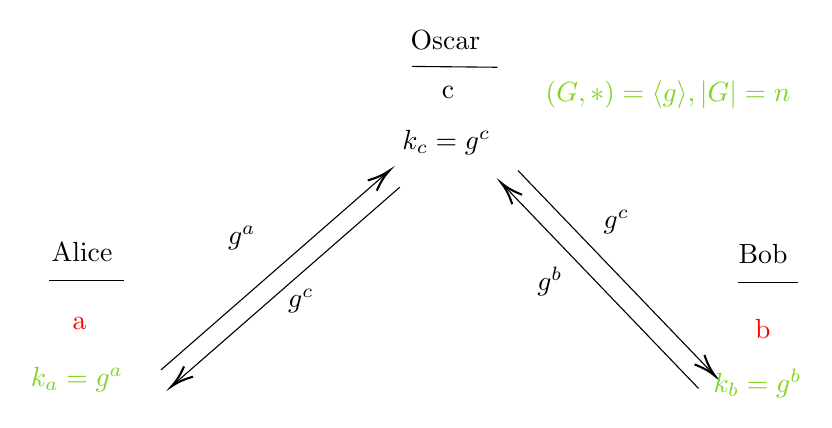
\begin{tikzpicture}[x=0.75pt,y=0.75pt,yscale=-1,xscale=1]
        \draw    (108,147.4) -- (144,147.4) ;
        \draw    (440,148.4) -- (469,148.4) ;
        \draw    (283,44.4) -- (324,44.8) ;
        \draw    (162,190.6) -- (270.49,95.92) ;
        \draw [shift={(272,94.6)}, rotate = 138.89] [color={rgb, 255:red, 0; green, 0; blue, 0 }  ][line width=0.75]    (10.93,-3.29) .. controls (6.95,-1.4) and (3.31,-0.3) .. (0,0) .. controls (3.31,0.3) and (6.95,1.4) .. (10.93,3.29)   ;
        \draw    (168.51,197.28) -- (277,102.6) ;
        \draw [shift={(167,198.6)}, rotate = 318.89] [color={rgb, 255:red, 0; green, 0; blue, 0 }  ][line width=0.75]    (10.93,-3.29) .. controls (6.95,-1.4) and (3.31,-0.3) .. (0,0) .. controls (3.31,0.3) and (6.95,1.4) .. (10.93,3.29)   ;
        \draw    (334,94.6) -- (427.62,192.16) ;
        \draw [shift={(429,193.6)}, rotate = 226.18] [color={rgb, 255:red, 0; green, 0; blue, 0 }  ][line width=0.75]    (10.93,-3.29) .. controls (6.95,-1.4) and (3.31,-0.3) .. (0,0) .. controls (3.31,0.3) and (6.95,1.4) .. (10.93,3.29)   ; 
        \draw    (327.38,102.04) -- (421,199.6) ;
        \draw [shift={(326,100.6)}, rotate = 46.18] [color={rgb, 255:red, 0; green, 0; blue, 0 }  ][line width=0.75]    (10.93,-3.29) .. controls (6.95,-1.4) and (3.31,-0.3) .. (0,0) .. controls (3.31,0.3) and (6.95,1.4) .. (10.93,3.29)   ;
        
        \draw (108,128) node [anchor=north west][inner sep=0.75pt]   [align=left] {Alice};
        \draw (439,129) node [anchor=north west][inner sep=0.75pt]   [align=left] {Bob};
        \draw (346,50) node [anchor=north west][inner sep=0.75pt]   [align=left] {\textcolor[rgb]{0.49,0.83,0.13}{$(G, *) = \langle g\rangle, |G| = n$}};
        \draw (281,26) node [anchor=north west][inner sep=0.75pt]   [align=left] {Oscar};
        \draw (118,164) node [anchor=north west][inner sep=0.75pt]   [align=left] {\textcolor[rgb]{1,0,0}{a}};
        \draw (98,188) node [anchor=north west][inner sep=0.75pt]   [align=left] {\textcolor[rgb]{0.49,0.83,0.13}{$k_a = g^a$}};
        \draw (447,165) node [anchor=north west][inner sep=0.75pt]   [align=left] {\textcolor[rgb]{1,0,0}{b}};
        \draw (427,189) node [anchor=north west][inner sep=0.75pt]   [align=left] {\textcolor[rgb]{0.49,0.83,0.13}{$k_b = g^b$}};
        \draw (277,74) node [anchor=north west][inner sep=0.75pt]   [align=left] {$k_c = g^c$};
        \draw (296,53) node [anchor=north west][inner sep=0.75pt]   [align=left] {c};
        \draw (193,120) node [anchor=north west][inner sep=0.75pt]   [align=left] {$g^a$};
        \draw (222,150.6) node [anchor=north west][inner sep=0.75pt]   [align=left] {$g^c$};
        \draw (374,112.6) node [anchor=north west][inner sep=0.75pt]   [align=left] {$g^c$};
        \draw (342,139.6) node [anchor=north west][inner sep=0.75pt]   [align=left] {$g^b$};
    \end{tikzpicture}
\end{center} 
In this scenario, Oscar has the capability to intercept the communication between Alice and Bob. Let's say Alice sends a message to Bob, but Oscar intercepts it and replaces it with a different message. For example, if Alice sends \( g^a \) to Bob, Oscar can calculate \( g^c \) since \( g \) and \( G \) are public. Oscar then sends \( g^c \) to Bob instead of \( g^a \). Since Bob lacks a means to verify the message's origin, he assumes it's from Alice, believing it to be her public key. However, in reality, Bob has received \( g^c \) instead of \( g^a \).\\
\\
When Bob shares his public key \( g^b \) with Alice, Oscar repeats the interception, sending \( g^c \) to Alice. Once again, Alice cannot verify the source of the message and accepts it.\\

\newline
Using the intercepted data, Alice can calculate \( (g^c)^a = g^{ac} \), Bob can calculate \( (g^c)^b = g^{bc} \), and Oscar can calculate \( (g^a)^c = g^{ac} \) and \( (g^b)^c = g^{bc} \) respectively. Consequently, Oscar possesses two shared secret keys: one identical to Alice's and the other to Bob's.
Unaware of Oscar's interference, Alice and Bob continue their communication. Suppose Alice sends a message to Bob under the assumption that their communication remains secure.

\begin{center}
    \tikzset{every picture/.style={line width=0.75pt}}     
    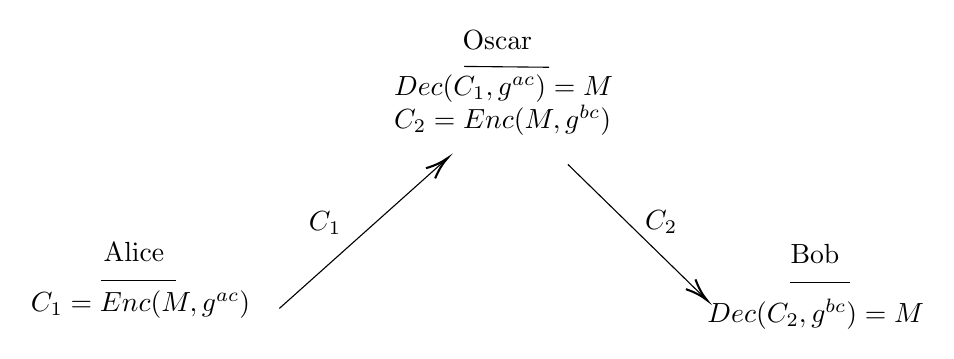
\begin{tikzpicture}[x=0.75pt,y=0.75pt,yscale=-1,xscale=1]
        \draw    (107,400.4) -- (143,400.4) ;
        \draw    (439,401.4) -- (468,401.4) ;
        \draw    (282,297.4) -- (323,297.8) ;
        \draw    (193,414) -- (272.51,342.93) ;
        \draw [shift={(274,341.6)}, rotate = 138.21] [color={rgb, 255:red, 0; green, 0; blue, 0 }  ][line width=0.75]    (10.93,-3.29) .. controls (6.95,-1.4) and (3.31,-0.3) .. (0,0) .. controls (3.31,0.3) and (6.95,1.4) .. (10.93,3.29)   ;
        \draw    (332,344.6) -- (397.57,408.6) ;
        \draw [shift={(399,410)}, rotate = 224.31] [color={rgb, 255:red, 0; green, 0; blue, 0 }  ][line width=0.75]    (10.93,-3.29) .. controls (6.95,-1.4) and (3.31,-0.3) .. (0,0) .. controls (3.31,0.3) and (6.95,1.4) .. (10.93,3.29)   ;
        
        \draw (107,381) node [anchor=north west][inner sep=0.75pt]   [align=left] {Alice};
        \draw (438,382) node [anchor=north west][inner sep=0.75pt]   [align=left] {Bob};
        \draw (280,279) node [anchor=north west][inner sep=0.75pt]   [align=left] {Oscar};
        \draw (206,366) node [anchor=north west][inner sep=0.75pt]   [align=left] {$C_1$};
        \draw (368,365.6) node [anchor=north west][inner sep=0.75pt]   [align=left] {$C_2$};
        \draw (247,300) node [anchor=north west][inner sep=0.75pt]   [align=left] {$Dec(C_1, g^{ac}) = M$\\$C_2 = Enc(M, g^{bc})$};
        \draw (72,404) node [anchor=north west][inner sep=0.75pt]   [align=left] {$C_1 = Enc(M, g^{ac})$};
        \draw (398,408) node [anchor=north west][inner sep=0.75pt]   [align=left] {$Dec(C_2, g^{bc}) = M$};
    \end{tikzpicture}
\end{center}

Alice encrypts the message using \( g^{ac} \) and sends it. Oscar intercepts this message and decrypts it using \( g^{ac} \), gaining access to the original message sent by Alice. Oscar then encrypts this message using \( g^{bc} \) and sends it to Bob. Upon receiving the message, Bob decrypts it using \( g^{bc} \) and perceives it as the original message sent by Alice. Unbeknownst to both Alice and Bob, Oscar has intercepted and manipulated their communication. This scenario represents a Man-in-the-Middle Attack on the Diffie-Hellman Key Exchange Algorithm.\\

In messaging platforms like WhatsApp or Telegram, Diffie-Hellman Key Exchange is utilized. However, this exchange occurs through the intermediary service provider (e.g., WhatsApp or Telegram), introducing potential vulnerabilities. While these service providers can manipulate the exchanged data if they choose, they typically implement security measures to safeguard the communication.\\

To compute the shared secret key \( g^{ab} \), it is necessary to compute \( g^a \) and \( g^b \) in a large group \( G \), with both \( a \) and \( b \) being sufficiently large. Since selecting any pseudo-random number between 1 and \( (n-1) \) is highly likely to fall within the middle range, if \( |G| = 2^{512} \), then \( a \) and \( b \) would typically be around 256 bits. The challenge lies in efficiently computing \( g^a \) and \( g^b \). Traditional methods such as using loops and direct multiplication by \( g \) in each iteration are impractical. Instead, the Square and Multiply Algorithm is employed. In this algorithm, to compute \( x^c \), where \( c \) is represented in binary as \( c_{l-1} \ldots c_1c_0 \), a more efficient approach is utilized.Then, \\
 \vspace{3mm}
$c = \Sigma_{i = 0}^{l-1} c_i \cdot 2^i$\\
\vspace{3mm}
$x^c = x^{\Sigma_{i = 0}^{l-1} c_i \cdot 2^i} = \Pi_{i = 0}^{l-1} x^{c_i \cdot 2^i}$\\
\vspace{3mm}
$x^c = x^{c_0\cdot 2^0}\hdots x^{c_{l-1}\cdot 2^{l-1}}$\\
These are just $log(c)$ multiplications, hence, we can compute $x^c$ in logarithmic time of c.
\begin{center}
    \begin{algorithm}
    \caption{Square and Multiply Algorithm to find $x^c$}
        \textbf{Input:} x and c\\
        Z = 1;\\
        \For{$i = l - 1$ to $N0$}{
            $Z = Z^2$;\\
            \If{$c_i == 1$}{
                Z = Z * x;\\
            }
        }
        return Z;
    \end{algorithm}
\end{center}

Let's illustrate an example and compute \(3^5\). Here, \(x = 3\) and \(c = 5\), represented as \(101_2\) in binary. Initially, \(Z = 1\) and \(i = 2\) (since \(l = 3\)). In the first iteration of the loop, \(Z = Z^2 = 1\), since \(c_2 = 1\), \(Z = Z * x = 3\). In the second iteration, \(Z = 3\), \(i = 1\), \(Z = Z^2 = 9\), as \(c_1 = 0\), \(Z\) remains unchanged. In the last iteration, \(Z = 9\), \(i = 0\), \(Z = Z^2 = 81\), since \(c_0 = 1\), \(Z = Z * x = 81 * 3 = 243\). Thus, \(Z = 243 = 3^5\).

Using the Square and Multiply Algorithm, \(g^a\) and \(g^b\) can be efficiently computed in \(O(\log(a))\) and \(O(\log(b))\) time complexity, respectively.\\
\newline

\begin{center}
    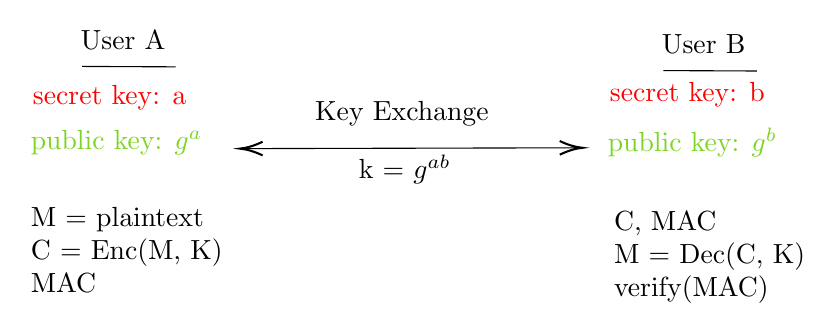
\begin{tikzpicture}[x=0.75pt,y=0.75pt,yscale=-1,xscale=1]
        \draw (161,476.4) -- (206,476.6) ;
        \draw (441,478.4) -- (486,478.6) ;
        \draw (239,516) -- (400,515.6) ;
        \draw [shift={(402,515.6)}, rotate = 179.86] [color={rgb, 255:red, 0; green, 0; blue, 0 } ][line width=0.75] (10.93,-3.29) .. controls (6.95,-1.4) and (3.31,-0.3) .. (0,0) .. controls (3.31,0.3) and (6.95,1.4) .. (10.93,3.29) ;
        \draw [shift={(237,516)}, rotate = 359.86] [color={rgb, 255:red, 0; green, 0; blue, 0 } ][line width=0.75] (10.93,-3.29) .. controls (6.95,-1.4) and (3.31,-0.3) .. (0,0) .. controls (3.31,0.3) and (6.95,1.4) .. (10.93,3.29) ;
        
        \draw (159,458) node [anchor=north west][inner sep=0.75pt] [align=left] {User A};
        \draw (136,484) node [anchor=north west][inner sep=0.75pt] [align=left] {\textcolor[rgb]{1,0,0}{secret key: a}};
        \draw (135,506) node [anchor=north west][inner sep=0.75pt] [align=left] {\textcolor[rgb]{0.49,0.83,0.13}{public key: $g^a$}};
        \draw (439,460) node [anchor=north west][inner sep=0.75pt] [align=left] {User B};
        \draw (414,483) node [anchor=north west][inner sep=0.75pt] [align=left] {\textcolor[rgb]{1,0,0}{secret key: b}};
        \draw (413,505) node [anchor=north west][inner sep=0.75pt] [align=left] {\textcolor[rgb]{0.49,0.83,0.13}{public key: $g^b$}};
        \draw (272,492) node [anchor=north west][inner sep=0.75pt] [align=left] {Key Exchange};
        \draw (293,518) node [anchor=north west][inner sep=0.75pt] [align=left] {k = $g^{ab}$};
        \draw (135,543) node [anchor=north west][inner sep=0.75pt] [align=left] {M = plaintext\\C = Enc(M, K)\\MAC};
        \draw (416,545) node [anchor=north west][inner sep=0.75pt] [align=left] {C, MAC\\M = Dec(C, K)\\verify(MAC)}; 
    \end{tikzpicture}
\end{center}
In the event of a Man-in-the-Middle Attack, it's essential to establish a communication setup that incorporates Message Authentication Codes (MAC). A MAC serves the dual purpose of verifying the message source and ensuring message integrity. By implementing MAC, we authenticate the source of the message, thereby mitigating the risk of a Man-in-the-Middle Attack.

\textbf{Explanation:}

A Man-in-the-Middle Attack occurs when an unauthorized third party intercepts and potentially alters communication between two parties. By introducing a Message Authentication Code (MAC) into the communication setup, we add an extra layer of security. The MAC acts as a cryptographic checksum, ensuring that the message originates from the expected source and hasn't been tampered with during transmission. Consequently, the inclusion of MAC prevents unauthorized intermediaries from intercepting and manipulating the communication undetected.


\subsection{RSA (Rivest Shamir Adleman) Encryption}
RSA (Rivest-Shamir-Adleman) Encryption is a fundamental public-key encryption algorithm. Before delving into RSA encryption, it's crucial to review some foundational concepts:

\begin{itemize}
  \item The Euler's Totient Function $\phi(n)$ determines the count of integers less than $n$ that are coprime to $n$. In other words, it represents the number of $x$ such that $\text{gcd}(x, n) = 1$, where $1 \leq x \leq n - 1$.
  
  \item Let's consider a set $S = \{x \mod m\}$, where $|S| = m$. All elements in set $S$ are unique, typically ranging from 0 to $m-1$. Assume an integer $a$ such that $\text{gcd}(a, m) = 1$. Now, suppose there exists another set $S_1$ defined as:
  \[ S_1 = \{ar_1 \mod m, ar_2 \mod m, \ldots, ar_m \mod m\} \]
  Since the elements $\{r_1, r_2, \ldots, r_m\}$ are distinct, and $\text{gcd}(a, m) = 1$, it can be inferred that $\{ar_1 \mod m, ar_2 \mod m, \ldots, ar_m \mod m\}$ will also consist of $m$ unique elements. This can be proven using contradiction. Suppose $ar_i = ar_j$ for $r_i \neq r_j$. Therefore:
  \[ ar_i \equiv ar_j \mod m \]
  As $\text{gcd}(a, m) = 1$, there exists an integer $b$ such that $ab \equiv 1 \mod m$ (from Bezout's Identity). This $b$ is termed the multiplicative inverse of $a$, calculable using the Extended Euclidean Algorithm. Therefore, multiplying both sides of the equation by $b$ yields:
  \[ b \cdot a \cdot r_i \equiv b \cdot a \cdot r_j \mod m \]
  \[ r_i \equiv r_j \mod m \quad (\because ab \equiv 1 \mod m) \]
  Hence, it contradicts the initial assumption that $r_i \neq r_j$. Thus, the elements in set $S_1$ are unique if and only if $\text{gcd}(a, m) = 1$.
\end{itemize}
\section{Euler’s Theorem}
If $\text{gcd}(a, m) = 1$, then $a^{\phi(m)} \equiv 1 \pmod{m}$.

Let's consider a set $S$ such that
\[ S = \{ x \mid \text{gcd}(x, m) = 1 \} \]
\[ S = \{s_1, s_2, s_3, s_4, \ldots, s_{\phi(m)} \} \]

Now, assuming $\text{gcd}(a, m) = 1$, let's create another set $S_1$ such that
\[ S_1 = \{ as_1, as_2, as_3, \ldots, as_{\phi(m)} \} \]

If $as_i \equiv as_j \pmod{m}$,
\[ \Rightarrow s_i \equiv s_j \pmod{m} \]

Given that $\text{gcd}(a, m) = 1$ and $b \cdot a \equiv 1 \pmod{m}$,
\[ |S| = \phi(m) \]
\[ |S_1| = \phi(m) \]

Since $a$ is coprime with $m$ and $s_i$ is also coprime with $m$, there must be some correspondence between elements of $S$ and $S_1$.
\[ s_i \equiv as_j \pmod{m} \]

Let's now take the product on both sides:
\[ \prod_{i=1}^{\phi(m)} s_i \equiv \prod_{j=1}^{\phi(m)} as_j \pmod{m} \]
\[ \Rightarrow \prod_{i=1}^{\phi(m)} s_i \equiv a^{\phi(m)} \cdot \prod_{j=1}^{\phi(m)} s_j \pmod{m} \]

Since $\text{gcd}(s_i, m) = 1$, each $s_i$ will have a multiplicative inverse under mod $m$. After simplification, we get:
\[ a^{\phi(m)} \equiv 1 \pmod{m} \]

\section{Fermat’s Theorem}
If $P$ is a prime number and $P$ does not divide $a$ (meaning that $P$ is coprime to $a$), then
\[ a^{P-1} \equiv 1 \pmod{P} \]

Using Fermat’s theorem,
\[ a^P \equiv a \pmod{P} \]

\textbf{Note:} If $P \mid a$ (where $P$ divides $a$), then
\[ a \equiv 0 \pmod{P} \]
\[ a^P \equiv 0 \pmod{P} \]
\[ a^P \equiv a \pmod{P} \]

However, Fermat’s theorem will not hold when $P$ divides $a$.

\section{RSA Cryptosystem}

\textbf{Facts:}
\begin{itemize}
    \item If $\text{gcd}(a, m) = 1$, then $a^{\phi(m)} \equiv 1 \pmod{m}$.
    \item If $P$ is a prime number, then $a^{P-1} \equiv 1 \pmod{P}$.
\end{itemize}

Now, let's understand the components of RSA:
\begin{enumerate}
    \item $n = pq$, where $p$ and $q$ are prime numbers.
    \item Plaintext space: $\mathbb{Z}_n$, Ciphertext space: $\mathbb{Z}_n$.
    \item Key space: $\{ K = (n,p,q,e,d) \mid ed \equiv 1 \pmod{\phi(n)} \}$.
    \item Encryption:
    \[ E(x, K) = c, \quad c = E(x, K) = x^e \pmod{n} \]
    \item Decryption:
    \[ \text{Dec}(c, K) = x, \quad c = \text{Dec}(c, K) = c^d \pmod{n} \]
\end{enumerate}

We know that $e$ and $d$ are related as:
\[ ed \equiv 1 \pmod{\phi(n)} \Rightarrow ed - 1 = t\cdot\phi(n) \Rightarrow 1 = ed + t\cdot\phi(n) \]

Encryption:
\[ c = x^e \pmod{n} \]

Decryption:
\[ x = c^d \pmod{n} \]
\[ c^d = (x^e)^d \mod n \]
\[ c^d = x^{ed} \mod n \]

Now using $ed = 1 + t\cdot\phi(n)$ from above:
\[ c^d = x^{1 + t\cdot\phi(n)} \mod n \]
\[ c^d = x \cdot x^{t\cdot\phi(n)} \mod n \]

Since $p$ and $q$ are primes and $n = pq$, then $\phi(n) = (p-1)(q-1)$:
\[ c^d = x \cdot x^{t[(p-1)(q-1)]} \mod (pq) \]

Now let us simplify the part $x^{t[(p-1)(q-1)]} \mod (pq)$, where $x \in \mathbb{Z}_n$:

We check $x^{t[(p-1)(q-1)]} \mod p$:
\[ \equiv x^{p-1} \mod p \equiv 1 \pmod p \] [As $x^{p-1} \equiv 1 \pmod p$]

We check $x^{t[(p-1)(q-1)]} \mod q$:
\[ \equiv x^{q-1} \mod q \equiv 1 \pmod q \] [As $x^{q-1} \equiv 1 \pmod q$]

Finally, we have:
\[ x^{t[(p-1)(q-1)]} \equiv 1 \pmod p \]
\[ x^{t[(p-1)(q-1)]} \equiv 1 \pmod q \]
\[ \Rightarrow x^{t[(p-1)(q-1)]} \equiv 1 \pmod {pq} \]

Substituting the above result:
\[ c^d = x \cdot 1 \mod (pq) \]
\[ c^d = x \mod (pq) \]

Hence, the decryption process is successful. Now, let's consider a scenario where Alice intends to communicate with Bob. In this scenario, two keys play pivotal roles: one is the public key, and the other is the secret key. Bob encrypts the message and sends it to Alice, who possesses both keys. While Bob is aware of the public key, he doesn't have access to the secret key.

\textbf{Alice:}
\begin{itemize}
    \item $n = pq$, where $p$ and $q$ are large prime numbers.
    \item $ed \equiv 1 \pmod{\phi(n)}$
    \item Alice selects $e$.
    \item Public key of Alice: $(n, e)$
    \item She computes $d$ using the extended Euclidean algorithm.
    \item Secret key of Alice: $(p, q, d)$
\end{itemize}

\textbf{Bob:}
\begin{itemize}
    \item Bob chooses a message $x$ from $\mathbb{Z}_n$.
    \item He knows $n$ and $e$ for Alice, allowing him to encrypt: $y = x^e \pmod{n}$
    \item Bob sends the encrypted message $y$ to Alice.
\end{itemize}

\textbf{Alice:}
\begin{itemize}
    \item Alice decrypts the message using her secret key: $x = y^d \pmod{n}$
\end{itemize}

If we are given $n$, how can we find $p$ and $q$ in polynomial time? We can iterate a loop from 2 to $\sqrt{n}$, and for each iteration, check if $n \% i$ equals zero. If it does, it means we have found a factor. Then, we verify if the factor is prime. If it is, we divide $n$ by $p$ to obtain $q$. However, finding the prime factors of a large number $n$ is a computationally hard problem.

\textbf{Note:} If we can compute $p$ and $q$ from $n$, we can also compute $\phi(n)$. Since we already have $e$, we can find $d$ using the extended Euclidean algorithm, thus compromising the security of RSA. Hence, RSA relies on the difficulty of the factorization problem.

\section{RSA Problem :-}
The RSA problem involves the challenge of deducing the plaintext $x$ given the public key $(n, e)$ and the ciphertext $c$ (where $c = x^e$). If one could efficiently derive $x$ from this information, the security of RSA would be compromised.\\

There's a misconception that there exists an algorithm capable of solving the RSA problem without requiring factorization. However, this is not true. It's essential to note that even if RSA can be broken, there's no guarantee that its factors can be determined. Conversely, if the factors are known, RSA can be broken, but the reverse isn't always valids.\\
 So RSA is secure under two assumptions:\\
• factorization is hard\\
• decryption is hard\\
It's noteworthy that public key encryption tends to be resource-intensive due to the exponentiation operations involved in $x^e$ and $c^d$. Consequently, such operations are typically avoided when possible.

\subsection*{Factorization Problem in RSA}

The factorization problem in the context of RSA encryption involves the challenge of finding the prime factors of a large composite number $n$ when only $n$ is known. In RSA, the security of the encryption scheme relies on the difficulty of factoring the product of two large prime numbers.\\

RSA encryption relies on the principle that it's easy to multiply two large prime numbers to obtain a large composite number, but it's computationally difficult to factorize the resulting composite number back into its prime factors. Specifically, given a composite number $n$ that is the product of two large primes $p$ and $q$ ($n = p \times q$), the factorization problem involves finding $p$ and $q$ when only $n$ is known.\\

The security of RSA encryption hinges on the assumption that factoring large composite numbers into their prime factors is a computationally intensive task, especially as the size of the primes increases. If an efficient algorithm were to be developed that could quickly factorize large composite numbers, it would render RSA encryption insecure, as an adversary could derive the private key $d$ from the public key $(n, e)$ and decrypt encrypted messages without authorization.\\

Therefore, the factorization problem of RSA refers to the difficulty of factoring a large composite number $n$ into its prime factors $p$ and $q$, which forms the basis of the security of the RSA encryption algorithm.

\sections{Digital Signature Algorithms}

Digital Signature Algorithms (DSA) play a crucial role in digitally signing documents and messages. When employing a DSA, only the signer is authorized to sign a document, but anyone can verify the signature. Formally, a DSA is defined as a tuple $(P, S, K, \text{Sign}, \text{V})$, where:

\begin{itemize}
    \item $P$: Plaintext
    \item $S$: Signature Text
    \item $K$: Key Space
    \item $\text{Sign}$: Signing Algorithm
    \item $\text{V}$: Verification Algorithm
\end{itemize}

The signing algorithm, denoted as $\text{Sign}(p, k)$, takes plaintext $p$ and a key $k$ from the key space to generate a signature $s$. On the other hand, the verification algorithm $\text{V}$ takes plaintext $p$, signature $s$, and key $k$ as inputs, and outputs $1$ if $s$ matches the signature generated for $p$ with key $k$, and $0$ otherwise.

One commonly used algorithm for digital signatures is the RSA Signature Algorithm.


\subsection{RSA Signature Algorithm}

\begin{center}
    \tikzset{every picture/.style={line width=0.75pt}} 
    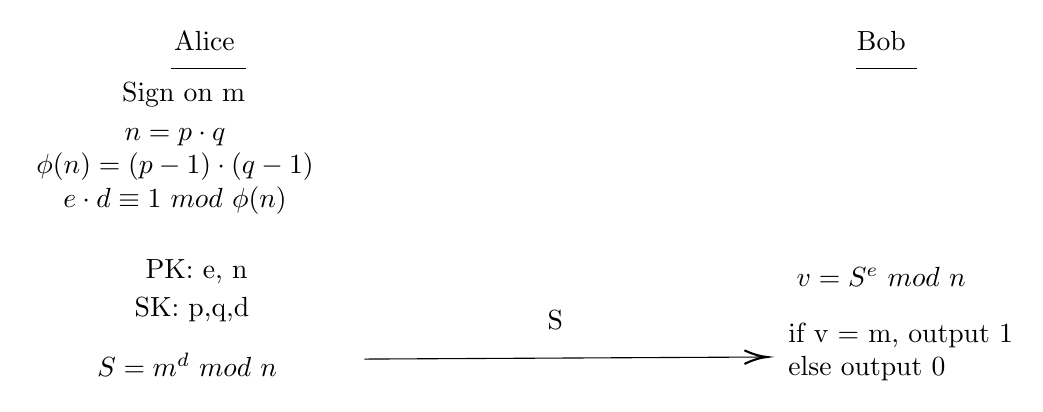
\begin{tikzpicture}[x=0.75pt,y=0.75pt,yscale=-1,xscale=1]

        \draw    (137,64.4) -- (173,64.4) ;
        \draw    (467,64.4) -- (496,64.4) ;
        \draw    (230,204.4) -- (422,203.41) ;
        \draw [shift={(424,203.4)}, rotate = 179.7] [color={rgb, 255:red, 0; green, 0; blue, 0 }  ][line width=0.75]    (10.93,-3.29) .. controls (6.95,-1.4) and (3.31,-0.3) .. (0,0) .. controls (3.31,0.3) and (6.95,1.4) .. (10.93,3.29)   ;
        
        \draw (137,45) node [anchor=north west][inner sep=0.75pt]   [align=left] {Alice};
        \draw (466,45) node [anchor=north west][inner sep=0.75pt]   [align=left] {Bob};
        \draw (112,70) node [anchor=north west][inner sep=0.75pt]   [align=left] {Sign on m};
        \draw (68,92) node [anchor=north west][inner sep=0.75pt]   [align=left] {\begin{minipage}[lt]{104.22pt}\setlength\topsep{0pt}
            \begin{center}
            $n = p \cdot q$\\$\phi(n) = (p-1)\cdot (q-1)$\\$e\cdot d \equiv 1\ mod \ \phi(n)$
            \end{center}
        \end{minipage}};

        \draw (118,155) node [anchor=north west][inner sep=0.75pt]   [align=left] {\begin{minipage}[lt]{44.68pt}\setlength\topsep{0pt}
            \begin{center}
            PK: e, n
            \end{center}
            SK: p,q,d
        \end{minipage}};
        \draw (100,200) node [anchor=north west][inner sep=0.75pt]   [align=left] {$S = m^d \ mod \ n$};
        \draw (317,180) node [anchor=north west][inner sep=0.75pt]   [align=left] {S};
        \draw (437,159) node [anchor=north west][inner sep=0.75pt]   [align=left] {$v = S^e \ mod \ n$};
        \draw (433,186) node [anchor=north west][inner sep=0.75pt]   [align=left] {if v = m, output 1\\else output 0};
    \end{tikzpicture}
\end{center}

Alice wishes to digitally sign a message \( m \), and Bob needs to verify Alice's digital signature. Alice begins by generating two large prime numbers, \( p \) and \( q \), which she will use to compute \( n = p \cdot q \) and \( \phi(n) = (p - 1) \cdot (q - 1) \). Next, Alice selects an integer \( e \) and computes \( d \) such that \( e \cdot d \equiv 1 \mod \phi(n) \). Using these parameters, Alice signs the message in a way that others can verify. Specifically, Alice computes:

\[
\text{Signing Algorithm: } S \equiv m^d \mod n
\]

Since \( d \) is Alice's secret key, only Alice can perform this computation. She then sends \( S \) to Bob. Bob computes \( v \equiv S^e \mod n \) using \( e \), which is Alice's public key. If \( v = m \), the output of the verification algorithm will be 1, indicating that the signature is verified. Otherwise, it will output 0. Note that Bob must know the message \( m \) for verification, which can be transferred using any encryption algorithm.\\

In RSA, during encryption, we compute \( y \equiv x^e \mod n \), using the public key of the receiver, while during decryption, we compute \( x \equiv y^d \mod n \), using the secret key of the receiver. However, in the RSA Signature Algorithm, during signing, we use the secret key of the signer (the person who signs), while during verification, we use the public key of the signer. This means that in the RSA Signature Algorithm, the computations are opposite to those in RSA encryption and decryption. In every Digital Signature Algorithm (DSA), signing is done using the secret key of the signer, and verification is done using the public key of the signer.
.\\

\subsection{RSA Encryption :- }
RSA encryption is a widely used cryptographic algorithm for securing digital communication. Let's delve into RSA encryption once more.

In RSA encryption, there are two sets of keys: the public key (PK) and the secret key (SK). The public key consists of \( n \) and \( e \), while the secret key consists of \( p \), \( q \), and \( d \). These values are computed as follows:

\[ n = p \cdot q \]

\[ \phi(n) = (p - 1) \cdot (q - 1) \]

\[ e \cdot d \equiv 1 \mod \phi(n) \]

The encryption process involves raising the message \( m \) to the power of \( e \) modulo \( n \), resulting in the ciphertext \( c \):

\[ c = m^e \mod n \]

When encrypting two different messages, \( m_1 \) and \( m_2 \), with RSA, we obtain two ciphertexts, \( c_1 \) and \( c_2 \). Multiplying these ciphertexts together yields a ciphertext for the product of the original messages:

\[ c_1 \cdot c_2 = (m_1 \cdot m_2)^e \mod n \]

This property allows for computation on encrypted data, enabling operations on the encrypted form of the messages without decryption.

However, addition of ciphertexts does not result in meaningful computation. But if a constant \( a \) is multiplied to the message \( m \) (with corresponding ciphertext \( c \)), the ciphertext for \( a \cdot m \) can be obtained without actual encryption. This multiplication is achieved by multiplying \( c \) with \( a^e \).

While RSA encryption does not support addition homomorphically, it facilitates multiplication homomorphically. Fully Homomorphic Encryption (FHE) algorithms enable both addition and multiplication operations on ciphertexts.

In the RSA Signature Algorithm, signatures on messages \( m_1 \) and \( m_2 \) are generated using the secret key:

\[ s_1 = m_1^d \mod n \]
\[ s_2 = m_2^d \mod n \]

Multiplying these signatures produces a signature for the product of the original messages:

\[ s_1 \cdot s_2 = (m_1 \cdot m_2)^d \mod n \]

This operation allows for computation on authenticated data, where the signature on the product of messages can be verified by others.

To prevent signature forgery, signatures are often computed on the hash of the message instead of the message itself. This ensures that forging a signature on a product of messages is not possible without knowing the secret key. The verification process involves comparing the computed value with the hashed message. Only with the public key of the signer can the message be verified.
\newline
\end{document}